\documentclass[onecolumn, draftclsnofoot,10pt, compsoc]{IEEEtran}

%slightly modified from stackoverflow @ https://tex.stackexchange.com/questions/200437/numbering-sections-subsections-etc-manually
%code block below allows for references to function as a section instead of a chapter
\makeatletter
\renewenvironment{thebibliography}[1]
{\subsection{References}
	\@mkboth{\MakeUppercase\bibname}{\MakeUppercase\bibname}%
	\list{\@biblabel{\@arabic\c@enumiv}}%
	{\settowidth\labelwidth{\@biblabel{#1}}%
		\leftmargin\labelwidth
		\advance\leftmargin\labelsep
		\@openbib@code
		\usecounter{enumiv}%
		\let\p@enumiv\@empty
		\renewcommand\theenumiv{\@arabic\c@enumiv}}%
%	\sloppy
	\clubpenalty4000
	\@clubpenalty \clubpenalty
	\widowpenalty4000%
	\sfcode`\.\@m}
{\def\@noitemerr
	{\@latex@warning{Empty `thebibliography' environment}}%
	\endlist}
\makeatother

\usepackage{graphicx}
\usepackage{url}
\usepackage{setspace}
\makeindex
\usepackage{geometry}

\geometry{textheight=9.5in, textwidth=7in}

% 1. Fill in these details
\def \CapstoneTeamName{		Wheelchair Data Collection Team}
\def \CapstoneTeamNumber{		4}
\def \GroupMemberOne{			Marie Bomber}
\def \GroupMemberTwo{			Aaron Leondar}
\def \GroupMemberThree{			Hadi Rahal-Arabi}
\def \CapstoneProjectName{			Robotic Wheelchair Data Collection and Analysis}
\def \CapstoneSponsorCompany{	Oregon State University}
\def \CapstoneSponsorPerson{	Matthew William Shuman	}

% 2. Uncomment the appropriate line below so that the document type works
\def \DocType{	%Problem Statement
				Requirements Document
				%Technology Review
				%Design Document
				%Progress Report
				}
\bibliographystyle{ieeetran}	
\newcommand{\NameSigPair}[1]{\par
\makebox[2.75in][r]{#1} \hfil 	\makebox[3.25in]{\makebox[2.25in]{\hrulefill} \hfill		\makebox[.75in]{\hrulefill}}
\par\vspace{-12pt} \textit{\tiny\noindent
\makebox[2.75in]{} \hfil		\makebox[3.25in]{\makebox[2.25in][r]{Signature} \hfill	\makebox[.75in][r]{Date}}}}
% 3. If the document is not to be signed, uncomment the RENEWcommand below
%\renewcommand{\NameSigPair}[1]{#1}

%%%%%%%%%%%%%%%%%%%%%%%%%%%%%%%%%%%%%%%
\begin{document}
\begin{titlepage}
    \pagenumbering{gobble}
    \begin{singlespace}
        \hfill 
        % 4. If you have a logo, use this includegraphics command to put it on the coversheet.
        %\includegraphics[height=4cm]{CompanyLogo}   
        \par\vspace{.2in}
        \centering
        \scshape{
            \huge CS Capstone \DocType \par
            {\large 27 October 2017}\par
            \vspace{.5in}
            \textbf{\Huge\CapstoneProjectName}\par
            \vfill
            {\large Prepared for}\par
            \Huge \CapstoneSponsorCompany\par
            \vspace{5pt}
            {\Large\NameSigPair{\CapstoneSponsorPerson}\par}
            {\large Prepared by }\par
            Group\CapstoneTeamNumber\par
            % 5. comment out the line below this one if you do not wish to name your team
            \CapstoneTeamName\par 
            \vspace{5pt}
            {\Large
                \NameSigPair{\GroupMemberOne}\par
                \NameSigPair{\GroupMemberTwo}\par
                \NameSigPair{\GroupMemberThree}\par
            }
            \vspace{20pt}
                    \begin{abstract}
            	% 6. Fill in your abstract    
This document will serve to provide the requirements for the Wheelchair Data Collection capstone project under Matthew Shuman. The document provides as a high-level description of the project, but does not discuss design or implementation. Our capstone will inherit constraints from the parent project at Oregon State University, Project Chiron. These constraints include privacy restrictions for wheelchair operators, visual interface requirements for the undergraduate tester, and simple data accessibility for the researcher.
            \end{abstract} 
        }   
    \end{singlespace}
\end{titlepage}
\newpage
\pagenumbering{arabic}
\tableofcontents
%\listoffigures
%\listoftables
\clearpage

% 8. now you write!
\section{Introduction}
\subsection{Purpose}
This requirements document is intended to define the critical features and functionality for a GUI based testing interface for ROS. It is intended to act as an agreement between the client Matthew Shuman and the developers, Marie Bomber, Aaron Leondar and Hadi Rahal-Arabi (and any other relevant stakeholders) to the promised functions and abilities of the testing interface. 
\subsection{Scope}
The intent of this project is to produce a general purpose interface to design and run tests on robots that run ROS. Within this scope is a specific use-case of an easy to use interface for Project Chiron research. This interface will  begin and record user tests, and allow testing data to be retrieved so a researcher can run POMDP analysis on the gathered results. This project will not cover the modifications made to the Project Chiron robot (a Perimobile wheelchair) and will not include any hardware work with the exception of documenting any already-existing hardware modifications. 

\subsection{Definitions, Acronyms and Abbreviations}
\begin{description}
\item [Researcher] \hfill \break Admin level user of the Robot Test Controller. The researcher is expected to have full access to all user testing data (including names)
\item [POMDP] \hfill \break Partially Observable Markov Decision Process. Per POMDP.org "This is a mathematical model that can capture the domain dynamics that include uncertainty in action effects and uncertainty in perceptual stimuli. Once a problem is captured as POMDP, it them becomes more amendable for solution using optimization techniques." \cite{1}
\item [ROS] \hfill \break Robot Operating System
\item [ROS Bag] \hfill \break Collection of ROS Topic data created by the ROSbag library during a user test
\item [ROS Topics] \hfill \break A feature of ROS that 'publishes' relevant robot data and one of the primary communication methods of ROS. \cite{3} Examples of ROS Topics include the movement of a robotic arm or the contents of a video camera 'eye'. 
\item [Tester] \hfil \break Mid level user of the Robot Test Controller. The tester is expected to be able to initiate a user test, but will not be able to retrieve all user data. (May be able to retrieve data via an ID, but will not have access to testee names).
\item [Test Participant] \hfill \break Individual who has no access to the Robot Testing Controller, but will have a name and/or ID entry and who will run a user test.
\item [User Test] \hfill \break Instance of a single navigation of the testing course. This test will produce a bag of test participant data that the Robot Test Controller must be able to store and retrieve.
\end{description}
\bibliography{Bibliography}
\subsection{Overview}
This software requirements specification document contains all of the constraints of the robot test controller. It can be used as a functional description for the necessary components of the project, without discussion of their design or implementation.


\section{Overall Description}
\subsection{Product Perspective}
\begin{itemize}
	\item Interactions with the robot to be tested must be done with ROS, as it is a standard of the parent project.
	\item There will be no development or addition of hardware, only documentation of existing Project Chiron hardware.
\end{itemize}
\subsection{Product Functions}
\subsubsection{Create a New Test}
\begin{itemize}
	\item The application must allow a researcher to create and name a new test
	\item Once the robot is selected, the application must populate available ROS topics on the robot
	\item The researcher must be able to enter the following testing data
	\subitem The IP of the robot to be tested
	\subitem Where the researcher would like test information to be stored
	\subitem What ROS topics to record
	\subitem What metadata to include in the test
	\subitem The names of test participants or the number of participants in the test
	\item Once topics are selected, the interface should provide an estimate of how large a ROSbag would be based on selected topics. This estimate must be in a size per minute of test format
\end{itemize}
\subsubsection{Run an Existing Test}
\begin{itemize}
	\item The application must allow a user to select and run a test based on the definitions of a previously created test
	\item Once the test is selected the tester must be able to select which test participant to record data under. This can be an ID or test participant name, based on the test definitions
	\item The tester must be able to select which test number to record (to allow a test participant to be tested multiple times)
	\item The application must report the current connection status to the robot
	\item The application must auto-populate metadata when possible (such as date/time of test)
	\item The application must report a test status, such as 'waiting to begin', 'initializing' or 'begin'.
	\item The application must allow the tester to begin and end tests.
\end{itemize}
\subsubsection{Export Test Data}
\begin{itemize}
	\item The researcher should be able to see a list of bags, sortable by trial date/time and name or ID of testee.
	\item It must be simple to replace names associated with bags with testee IDs, to maintain data integrity but provide confidentiality to the testers.
	\item The core system should be able to accept a collected bag and correlate it with input from the user interface to create a data entry.
	\subitem The system should recognize if the user entered is a new testee or previous testee and link the new test to previous information.
	\item When passed a request from the user interface, the core system should pass the query to the main storage medium and return from the query in a format that meets the User Interface needs.
	\item The core system should securely store user logins and accept login requests so the interface only requires to handle pass/no pass scenarios.
\end{itemize}
\subsubsection{Wheelchair to Application Communication}
\begin{itemize}
	\item Application must connect with the wireless network of the robot.
	\item Application must be able to collect the list of tasks that the robot has available
	\item The bags, when stored, must also have relevant metadata. Examples of metadata include:
	\subitem The length of time of the trial.
	\subitem The date and time the trial was performed.
	\subitem the ID of the participant.
\end{itemize}
\subsubsection{Data Storage}
\begin{itemize}
	\item The system must recognize two levels of user access.
	\subitem Researcher - This level will have full access to user data, including test participant name and/or ID link.
	\subsubitem This level will also be able to delete the link between test participant name and test data at the researchers discretion
	\subitem Tester - This level has the ability to enter a testee name and start and end a test, but not have access to bag data.
\end{itemize}
\subsubsection{System Documentation}
\begin{itemize}

	\item Wiring for the testing hardware must be diagrammed so that the system could be recreated. 
	\item Structure of hardware system documentation must be at a level that an electrical engineer can recreate the system
		\subitem Once documentation is completed, it must meet researcher satisfaction
	\item All system software must be documented so a software engineer can install and run the application on a new system with no issues. 
		\subitem To test, software must be installed by 3 senior software engineering students in a new environment without error. 
\end{itemize}
\subsection{User Characteristics}
\begin{itemize}
	\item The user of the recording interface will be an unaffiliated paid undergraduate student, as such the collector must have a simple button interface for recording data.
	\item The users receiving the bag will be researchers affiliated with the robotic research, as such access to the bags should be trivial, but authenticated

\end{itemize}
\subsection{Constraints}
\begin{itemize}
	\item The data entry must be stored in a secure storage space that complies with the Institutional Review Board as defined by the client.
		\subitem Testee names must be separate from a unique ID.
		\subitem The reference link between testee names and ID's must be able to be purged at the client's request.
	\item All testing hardware must be recorded with part numbers and pricing.
	\item The tester should experience little latency (less than 500ms) when sorting bags in the interface.
	\item The researcher must have a method of exporting bags, or accessing bags outside of the interface.
	\item The interface must be portable, both capable of running externally on a server, or locally.
	\item Bags cannot contain more than strictly required data because all bags must fit on a moderately-sized flash drive (no more than 16GB).
\end{itemize}
\subsection{Assumptions and Dependencies}
\begin{itemize}
	\item Changes to the parent project may impact requirements of the robot test collector interface.
	\item The bag files should be appropriately sized to facilitate portable storage of roughly 100 trial runs.
	\begin{figure}[h!]
		
		\centering
		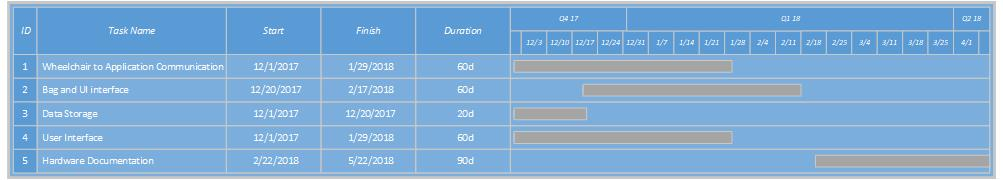
\includegraphics[width=\linewidth, scale=0.7]{PrelimGanttChart.jpg}
		Figure 1. The deadlines above are dependent on The Project Chiron research timeline
	\end{figure}
	
\end{itemize}



\end{document}